\newpage
\section{NGS}

\paragraph*{Problems with Sanger DNA sequencing}

\begin{enumerate}
  \item \textbf{Sensitivity} - Sanger technology, as well as other
technologies, do not allow to read the signal from a single DNA
molecule. Therefore, the fragment of DNA to be sequenced
must be amplified and the signal is obtained from many
identical fragments. This requires \textbf{bacterial cloning}.
A very major bottleneck.
  \item \textbf{Electrophoresis} - Sanger technology
requires the separation of the sequencing
reaction by individual electrophoresis, which
is another major bottleneck of the technology.
\end{enumerate}


To prepare a NGS libraries you need to have DNA fragments and some adapters,
and you need to attach Adapters to DNA fragments (see figure \ref{fig:ngs})

\begin{figure}[H]
  \centering
  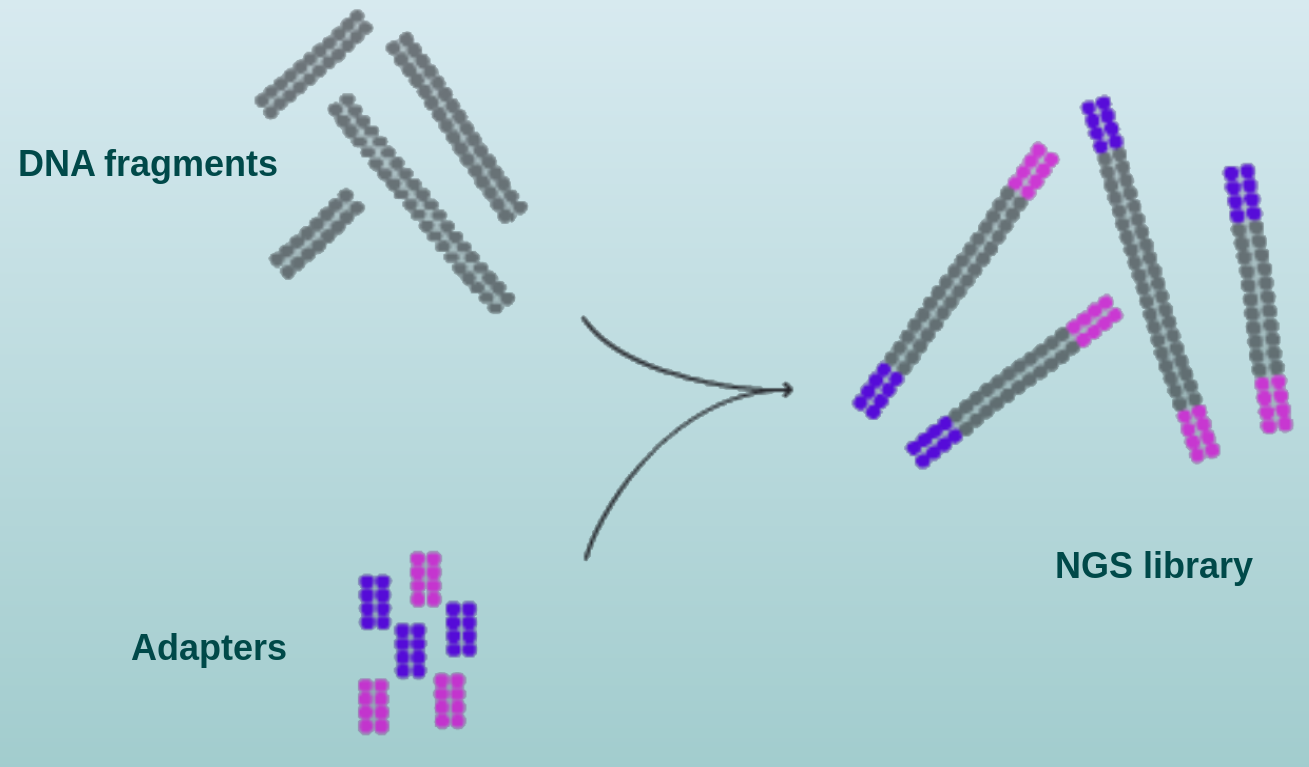
\includegraphics[scale=0.2]{ngs}
  \caption{Preparation of NGS libraries}
  \label{fig:ngs}
\end{figure}

NGS doesn't use cloning in bacteria, but use PCR - Colonies (Polonies), so DNA
is not mixed.

\textbf{Emulsion PCR} (ePCR) is a PCR variation that some NGS technologies use
to replicate DNA sequences.
It is conducted on a bead surface within tiny water bubbles floating on an oil
solution.

\begin{figure}[H]
  \centering
  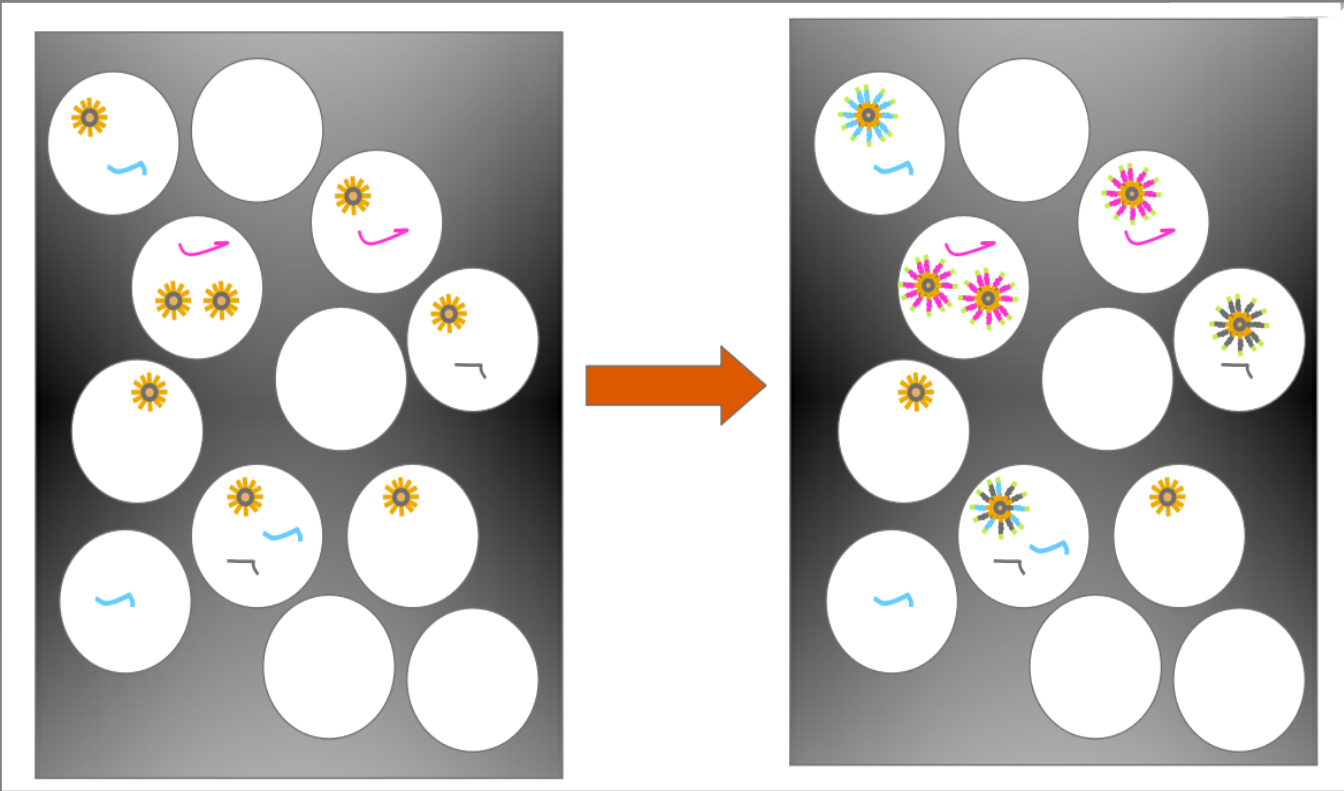
\includegraphics[scale=0.2]{epcr}
\end{figure}

\paragraph*{Why replicate DNA?}

This is a very important concept to understand, as all NGS techniques replicate
DNA before sequencing is done.

In short, DNA is replicated in order to amplify signals. No matter the method
of sequencing, without a proper amount of amplification, it's near impossible
to detect each base call. \\

NGS doesn't need electrophoresis, but it uses istead different methods
like the Pyrosequencing, that uses ATP and Luciferase, or Illumina
chemistry (which is the most used method today).

\subsection{Single-end reads and paired-end reads}

NGS sequencing can be done with single-end reads or paired-end reads.

\paragraph*{Sequencing in one or two directions}

DNA fragments used in the sequencing libraries are selected until a fixed
length.
Sequencing can start from only one end (\textbf{single-end sequencing})
or both the extremities of the fragments (\textbf{paired-end sequencing})
- and then it goes in opposite directions.

\paragraph*{Paired-end sequencing}
Paired-end sequencing is more accurate than single-read sequencing.
It makes easier the process of alignment and it allows to detect deletions,
duplications or insertions.

Tipically the two reads produced are not complementary and not overlapping
because the don't cover the whole length of the starting fragment.

The missing sequence is unknown, but what its length is given.

\textbf{Example}

\begin{figure}[H]
  \centering
  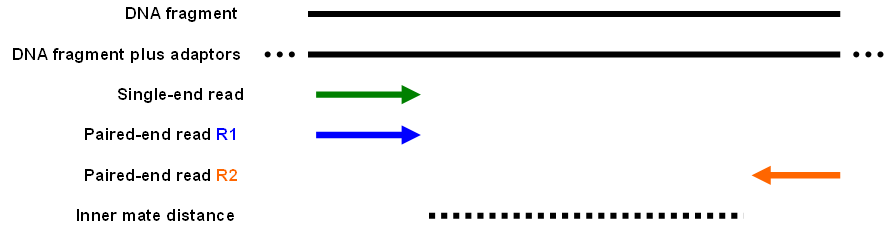
\includegraphics[scale=0.43]{sequencing}
  \caption{Starting from the top, a DNA fragment, DNA fragment plus adaptors,
single-end read, paired-end reads R1 R2, inner mate distance}
  \label{fig:sequencing}
\end{figure}

In the example, we expect that when aligning the two reads R1 R2 with the
reference genome, the distance between them (\textit{inner mate distance})
remains the same.

\textbf{If we see that R1 and R2 match at a greater or lower distance, we
deduce that there has been a deletion or a insertion (respectively)}.\\

\textbf{Mate pair sequencing} is a variant of paired-end sequencing.

